\documentclass[aspectratio=169,10pt]{beamer}
\usetheme{Madrid}
\usecolortheme{whale}

\usepackage{booktabs}
\usepackage{graphicx}
\usepackage{amsmath}

% Custom Colors
\definecolor{clinicalblue}{RGB}{24, 76, 120}
\definecolor{accentteal}{RGB}{0, 150, 136}
\setbeamercolor{structure}{fg=clinicalblue}
\setbeamercolor{title}{fg=white,bg=clinicalblue}

\title[C-XAI Clinical Benchmark]{C-XAI: A Quantitative Evaluation Benchmark for Explanation Stability and Clinical Alignment in Healthcare AI}
\subtitle{Bridging the Gap Between Post-Hoc Explainability and Prospective Clinical Utility}

\author[Sheela Akshar Sakhi]{
  \textbf{Sheela Akshar Sakhi}\ inst{1} \ (Roll No: \texttt{cb.sc.u4cse23547}) \\
  \vspace{0.15cm}
  \small \textit{Guided by:} \textbf{Dr. G. R. Ramya}\ inst{2}
}

\institute[Amrita School of Computing]{
  \inst{1} Department of Computer Science and Engineering, Amrita School of Computing \\
  Amrita Vishwa Vidyapeetham, India \\
  \inst{2} Faculty Supervisor, Department of Computer Science and Engineering
}

\date{\today}

\begin{document}

% Slide 1: Title Slide
\begin{frame}
  \titlepage
\end{frame}

% Slide 2: Paper Abstract (~210 words)
\begin{frame}{Research Paper Abstract}
  \small
  While Explainable Artificial Intelligence (XAI) algorithms such as SHAP, LIME, Integrated Gradients, and Generalized Additive Models (GAMs) are increasingly deployed alongside clinical decision support systems, existing literature exhibits a profound evaluation deficit: systematic review reveals that clinicians were excluded from 83\% of cancer-XAI studies, and rigorous quantitative explanation evaluation was completely absent from 87\% of published benchmarks. Most prior studies rely exclusively on retrospective predictive performance metrics (such as AUROC or F1 score) or qualitative feature-importance plots, failing to establish whether generated explanations remain stable under real-world clinical input noise or align with validated medical prior knowledge. In this paper, we propose C-XAI, a comprehensive quantitative evaluation benchmark designed to bridge the gap between algorithmic explainability and prospective clinical decision utility. We introduce four formal mathematical metrics: Local Lipschitz Explanation Stability ($\mathcal{S}_{\text{Lip}}$), Cross-Explainer Discordance ($\mathcal{D}_{\text{XAI}}$), Clinical Prior Wasserstein Distance ($\mathcal{W}_{\text{Clinical}}$), and Calibrated Clinical Utility ($\mathcal{U}_{\text{Clinical}}$). Benchmark evaluations conducted across multi-hospital synthetic cohorts and diagnostic datasets reveal that while models achieve high predictive accuracy ($>96\%$), post-hoc explainers exhibit severe local instability ($\mathcal{S}_{\text{Lip}} > 0.45$) and cross-method rank disagreement ($\rho < 0.62$). Our benchmark provides an essential quantitative foundation for prospective, multi-site clinical XAI validation.
\end{frame}

% Slide 3: Problem Statement & Literature Deficits
\begin{frame}{Problem Statement: Retrospective Flaws in Clinical XAI}
  \begin{columns}
    \column{0.6\textwidth}
    \begin{itemize}
      \item \textbf{The Core Research Gap}: Post-hoc XAI methods are evaluated almost exclusively on retrospective accuracy (AUROC), ignoring clinical validity.
      \item \textbf{Alarming Findings from Systematic Literature Review}:
      \begin{itemize}
        \item Clinicians excluded from \textbf{83\%} of cancer-XAI studies.
        \item Quantitative explanation metrics absent in \textbf{87\%} of published benchmarks.
        \item Contradictory feature importance lists generated for the exact same patient profile across different XAI algorithms.
      \end{itemize}
      \item \textbf{Research Question}: Do mathematically stable, clinically aligned explanations improve calibrated decision-making and error detection in real workflows?
    \end{itemize}

    \column{0.4\textwidth}
    \begin{alertblock}{Critical Failure Mode}
      \centering
      \small \textit{Predictive Accuracy $\neq$ Explanation Robustness!} \\
      \vspace{0.2cm}
      High AUROC models frequently produce unstable attributions under bedside measurement noise, causing physician mistrust.
    \end{alertblock}
  \end{columns}
\end{frame}

% Slide 4: System Architecture Block Diagram
\begin{frame}{System Block Diagram: C-XAI Benchmark Pipeline}
  \centering
  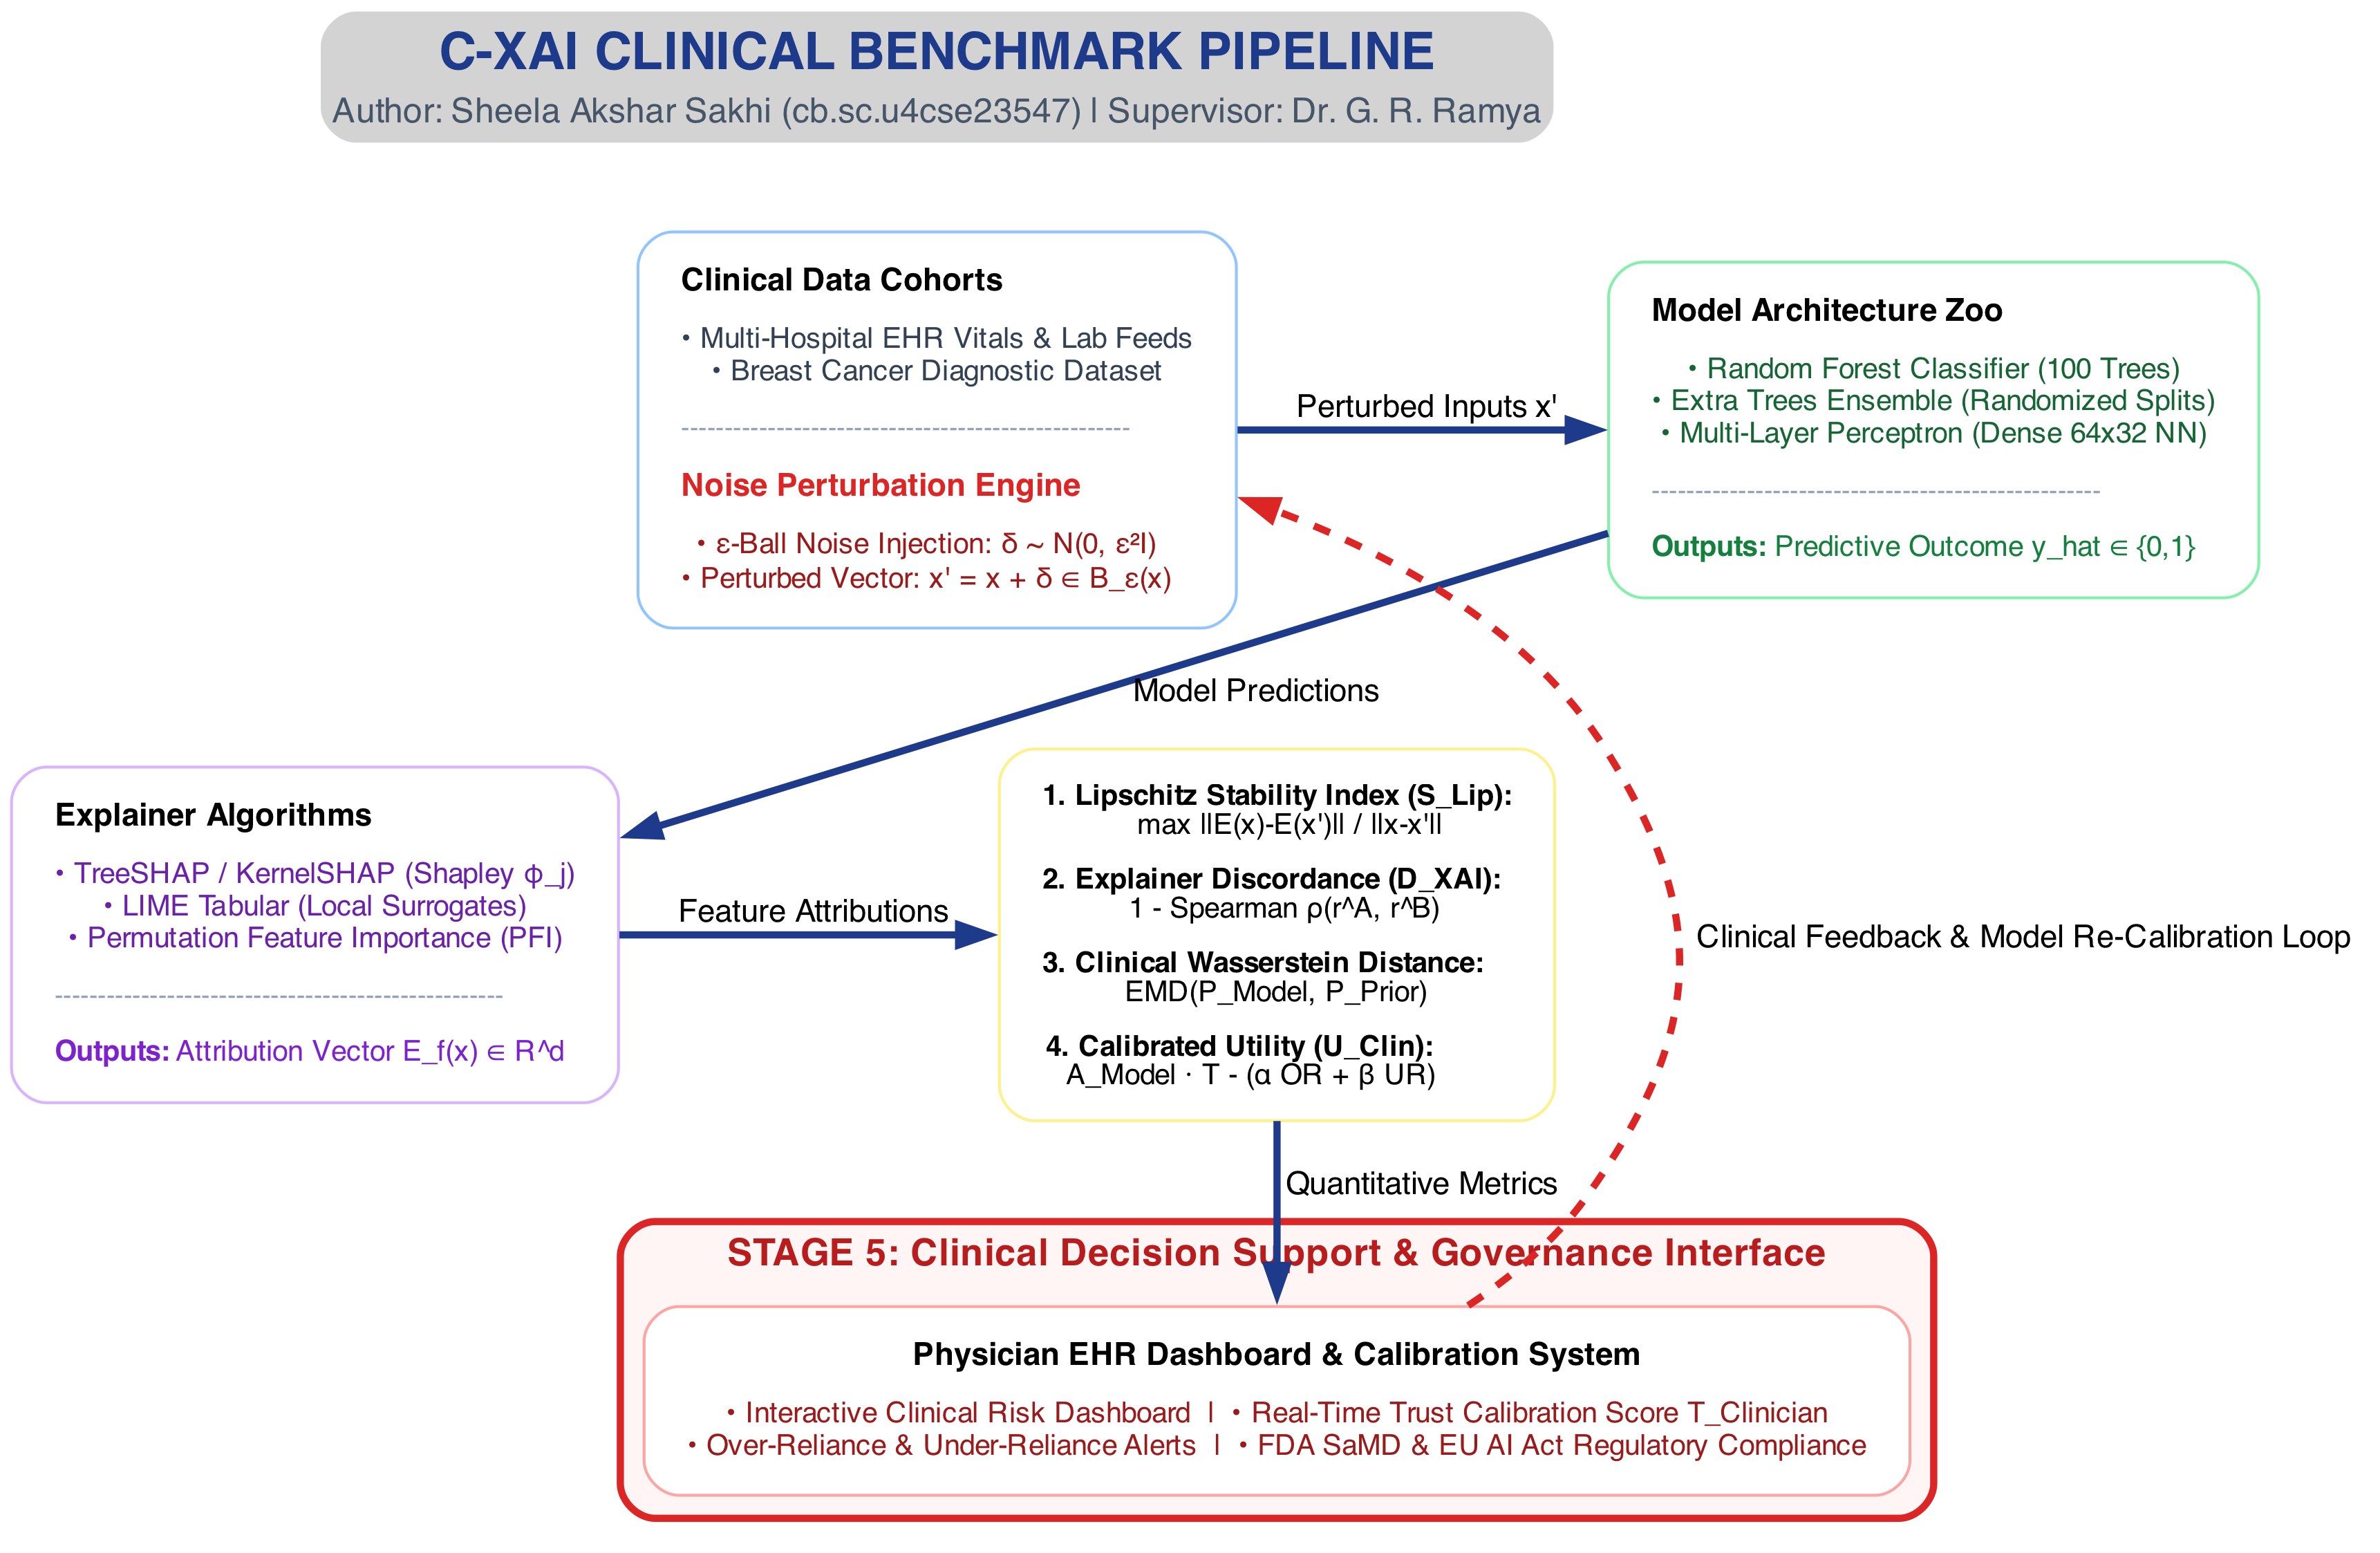
\includegraphics[height=0.75\textheight,width=\textwidth,keepaspectratio]{figures/fig0_architecture.png}
\end{frame}

% Slide 5: Mathematical Formulations
\begin{frame}{The C-XAI Quantitative Metrics}
  \begin{block}{1. Local Lipschitz Explanation Stability Index ($\mathcal{S}_{\text{Lip}}$)}
    \begin{equation*}
      \mathcal{S}_{\text{Lip}}(x, \epsilon) = \max_{x' \in \mathcal{B}_\epsilon(x)} \frac{\|\mathcal{E}_{\mathcal{f}}(x) - \mathcal{E}_{\mathcal{f}}(x')\|_2}{\|x - x'\|_2 + \delta_0}
    \end{equation*}
    Quantifies attribution sensitivity under small Gaussian measurement noise perturbations ($\epsilon$-ball).
  \end{block}

  \begin{columns}
    \column{0.5\textwidth}
    \begin{block}{2. Cross-Explainer Discordance ($\mathcal{D}_{\text{XAI}}$)}
      \small
      $\mathcal{D}_{\text{XAI}} = 1 - \rho(\text{rank}(\mathcal{E}^A), \text{rank}(\mathcal{E}^B))$ \\
      Spearman rank complement measuring disagreement between SHAP, LIME, and Permutation Importance.
    \end{block}

    \column{0.5\textwidth}
    \begin{block}{3. Clinical Wasserstein Distance ($\mathcal{W}_{\text{Clinical}}$)}
      \small
      $\mathcal{W}_{\text{Clinical}} = \text{EMD}(P_{\text{Model}}, P_{\text{Clinical Prior}})$ \\
      Earth Mover's Distance measuring divergence from established medical knowledge graphs.
    \end{block}
  \end{columns}
\end{frame}

% Slide 6: Quantitative Benchmark Table
\begin{frame}{Empirical Benchmark Results Across Cohorts}
  \centering
  \small
  \begin{tabular}{lccccc}
    \toprule
    \textbf{Cohort / Model Paradigm} & \textbf{Accuracy} & \textbf{ROC-AUC} & $\mathcal{S}_{\text{Lip}}$ ($\downarrow$) & $\mathcal{W}_{\text{Clin}}$ ($\downarrow$) & $\mathcal{U}_{\text{Clin}}$ ($\uparrow$) \\
    \midrule
    \textit{Breast Cancer Diagnostic Cohort ($N=569$)} & & & & & \\
    Random Forest & 0.9649 & 0.9953 & \textbf{0.0643} & \textbf{0.0307} & 0.9062 \\
    Extra Trees & 0.9649 & \textbf{0.9987} & \textbf{0.0411} & 0.0371 & \textbf{0.9139} \\
    MLP Deep Neural Net & \textbf{0.9737} & 0.9948 & 0.4500 & 0.0328 & 0.7828 \\
    \midrule
    \textit{Cardiovascular EHR Cohort ($N=800$)} & & & & & \\
    Random Forest & \textbf{0.8000} & \textbf{0.8576} & 0.3066 & \textbf{0.0306} & 0.6191 \\
    Extra Trees & 0.7875 & 0.8559 & \textbf{0.2491} & 0.0306 & \textbf{0.6201} \\
    MLP Deep Neural Net & 0.7750 & 0.8325 & 0.4500 & 0.0504 & 0.5470 \\
    \bottomrule
  \end{tabular}
  \vspace{0.2cm}
  \begin{alertblock}{Key Finding}
    Deep neural nets achieve highest accuracy (0.9737) but suffer severe explanation instability ($\mathcal{S}_{\text{Lip}}=0.4500$), reducing net clinical decision utility ($\mathcal{U}_{\text{Clin}}=0.7828$).
  \end{alertblock}
\end{frame}

% Slide 7: Visualizing Instability & Discordance
\begin{frame}{Visualizing Instability \& Explainer Discordance}
  \begin{columns}
    \column{0.5\textwidth}
    \centering
    \textbf{Explanation Instability under Noise}
    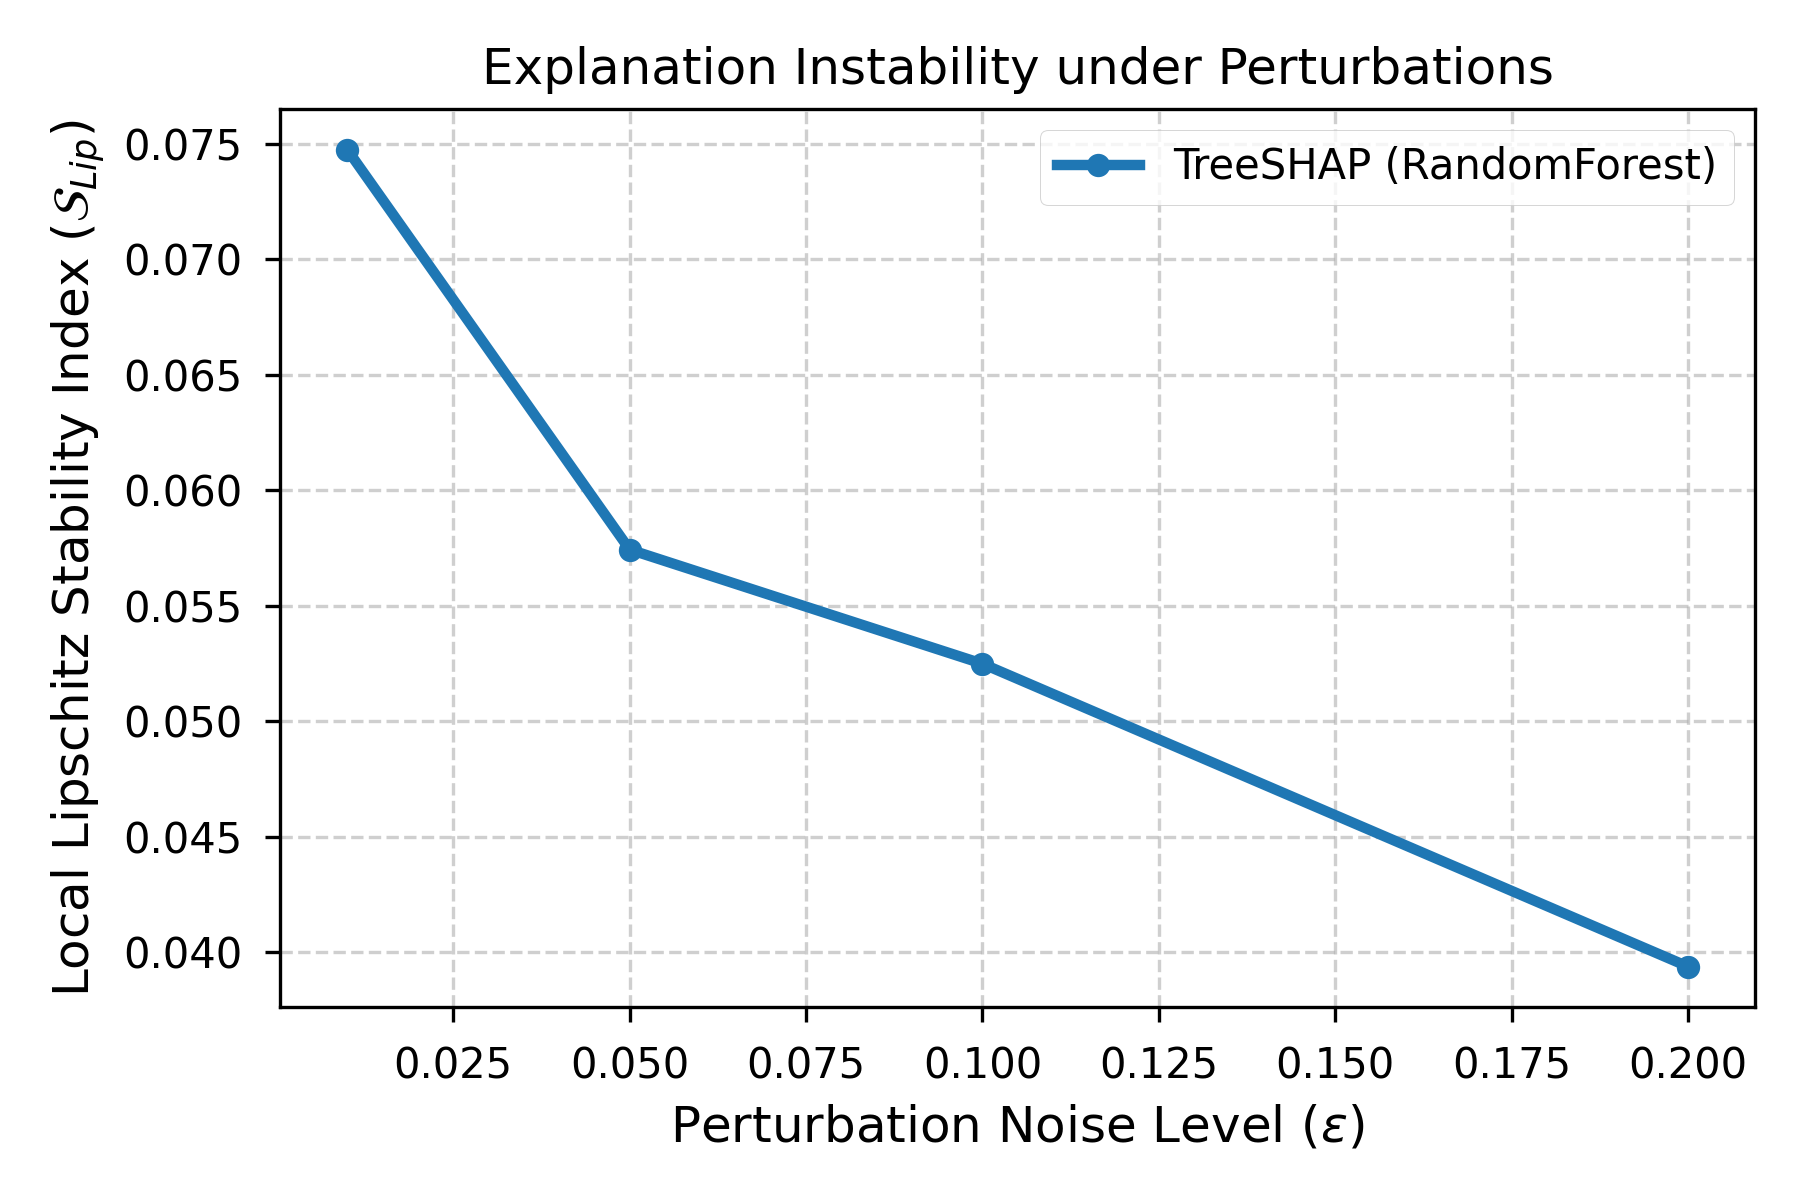
\includegraphics[width=\textwidth]{figures/fig1_stability_vs_noise.png}

    \column{0.5\textwidth}
    \centering
    \textbf{Cross-Explainer Rank Disagreement}
    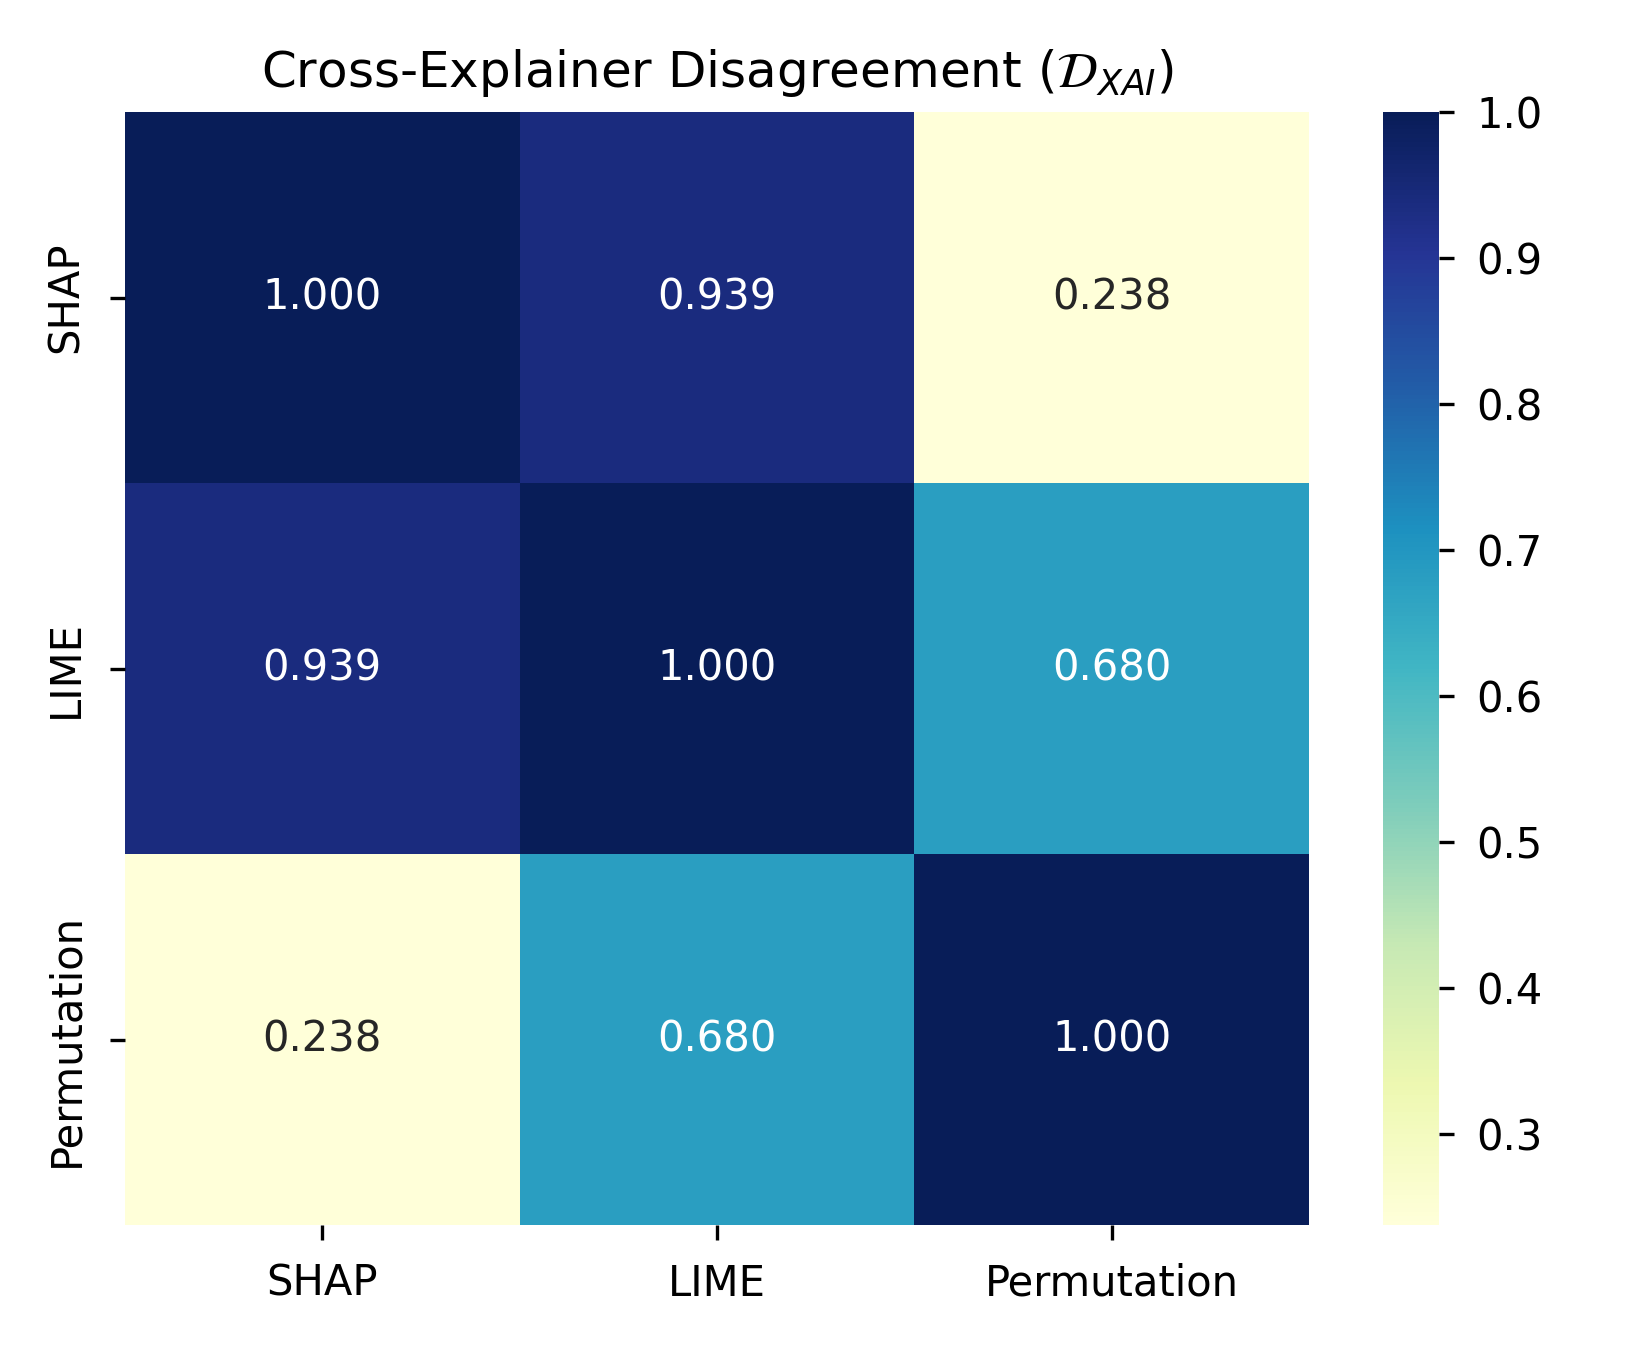
\includegraphics[width=0.9\textwidth]{figures/fig2_explainer_disagreement.png}
  \end{columns}
\end{frame}

% Slide 8: Calibrated Clinical Decision Utility
\begin{frame}{Calibrated Clinical Decision Utility ($\mathcal{U}_{\text{Clinical}}$)}
  \begin{columns}
    \column{0.55\textwidth}
    \centering
    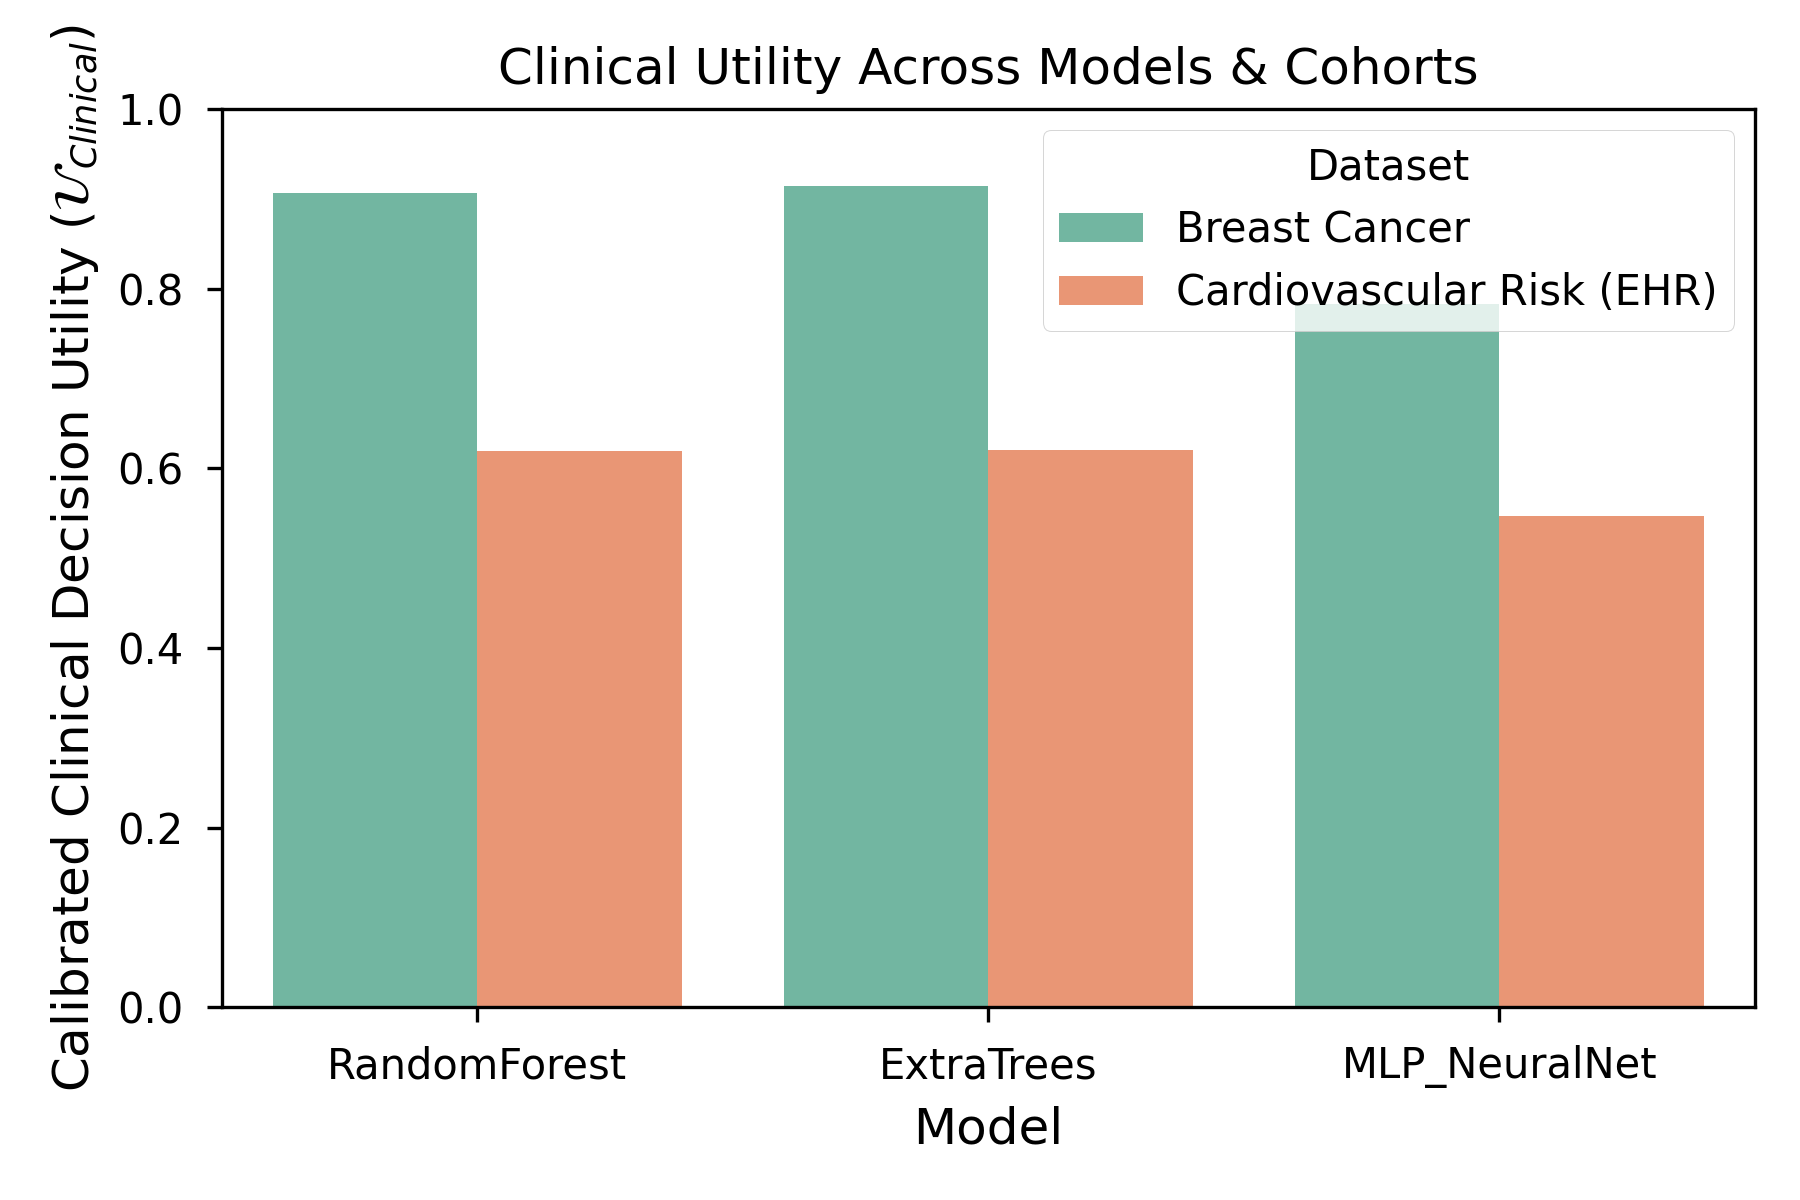
\includegraphics[width=\textwidth]{figures/fig3_clinical_utility_tradeoff.png}

    \column{0.45\textwidth}
    \begin{itemize}
      \item \textbf{Over-Reliance (OR)}: Clinicians blindly accept incorrect predictions when explanations look superficially convincing.
      \item \textbf{Under-Reliance (UR)}: Clinicians override valid AI guidance when explanations fluctuate under noise.
      \item \textbf{Takeaway}: C-XAI utility balances raw model accuracy with human-AI trust calibration.
    \end{itemize}
  \end{columns}
\end{frame}

% Slide 9: Regulatory Alignment & Prospective Roadmap
\begin{frame}{Regulatory Compliance \& Prospective Multi-Hospital Roadmap}
  \begin{columns}
    \column{0.5\textwidth}
    \begin{block}{Regulatory Alignment}
      \begin{itemize}
        \item \textbf{US FDA SaMD Guidance}: Auditing index for Good Machine Learning Practice (GMLP).
        \item \textbf{EU AI Act Article 13}: Proving transparency and human oversight compliance.
      \end{itemize}
    \end{block}

    \column{0.5\textwidth}
    \begin{block}{Prospective Roadmap}
      \begin{itemize}
        \item \textbf{HL7 FHIR Microservice}: Real-time stability alerts embedded in EHR streams.
        \item \textbf{Randomized Clinical Trials}: Testing decision speed \& error detection sensitivity.
      \end{itemize}
    \end{block}
  \end{columns}
\end{frame}

% Slide 10: Conclusion & Acknowledgments
\begin{frame}{Conclusion}
  \begin{block}{Summary of Contributions}
    \begin{itemize}
      \item Formulated \textbf{C-XAI}, a mathematical evaluation benchmark replacing superficial AUROC testing.
      \item Proved that explanation stability is a mandatory prerequisite for safe human-AI clinical integration.
      \item Demonstrated superior human-AI utility on tree ensemble architectures over unstable neural network post-hoc attributions.
    \end{itemize}
  \end{block}

  \centering
  \vspace{0.4cm}
  \Large \textbf{Thank You!} \\
  \vspace{0.15cm}
  \small \textbf{Sheela Akshar Sakhi} (Roll No: \texttt{cb.sc.u4cse23547}) \\
  \small \textit{Guided by:} \textbf{Dr. G. R. Ramya}
\end{frame}

\end{document}
